Ahora, con todas las partes del sistema convenientemente dispuestas y calibradas, procedimos a realizar las primeras medidas.

Hay que tener en cuenta que en estas primeras medidas no necesitamos un sistema de control de temperatura, ya que vamos a utilizar PMT y estos no son tan sensibles a la temperatura como los SiPM. Únicamente deberemos ser capaces de evitar oscilaciones grandes de temperatura ($\Delta T=15-20~\celsius$), los cuales sí afectan de forma apreciable a la ganancia del PMT. Esto lo podemos conseguir manteniendo el aire acondicionado de la sala experimental encendido y programado a una misma temperatura durante las medidas. 

Sin embargo, cuando vayamos a realizar las medidas del prototipo con SiPMs, si necesitaremos este control exhaustivo de la temperatura, ya que, como se vió en la sección de calibrado del SiPM, \ref{sec:Temperatura}, existe una dependencia muy marcada. Se necesitará adquirir un sistema de control de temperatura o, en su defecto, como construir y calibrar uno nosotros mismos.

La primera medida se realizó sin coincidencia, pasando directamente la señal 1 al MCA, el cual nos permite obtener un histograma energético.

Se obtuvo un primer histograma del prototipo con agua hiperpura y sin tritio. Dado que el agua hiperpura idealmente no añade ningun tipo de contribución al histograma llamaremos a esta medida señal de fondo. 

Seguidamente se rellenó el prototipo con agua tritiada y se obtuvo un segundo histograma. En esta segunda medida se pudo observar en el display del MCA que el número de cuentas medidas por segundo era mayor que el de la medida del fondo. Esto es un indicativo de que estamos detectando tritio. 

Finalmente se normalizaron cada uno de los histogramas al tiempo correspondiente a su medida para obtener histogramas de actividad en lugar de un histograma de sucesos. Los tiempos asociados al histograma del tritio y del fondo son $T_S=154143~\second$  y $T_B=246987~\second$, respectivamente, medidas largas para tener suficiente estadística. El resultado puede verse en la figura~\ref{senaltritio} izquierda. Además, se ha añadido una segunda imagen, figura\ref{senaltritio} derecha,  la cual se ha realizado representado la señal con tritio a la cual se le ha substraído la señal de fondo, es decir, en esta segunda imagen encontramos la señal debida únicamente al tritio.

\begin{figure}[htb]
\centering
{
%\subfloat[Espectro de emisión]
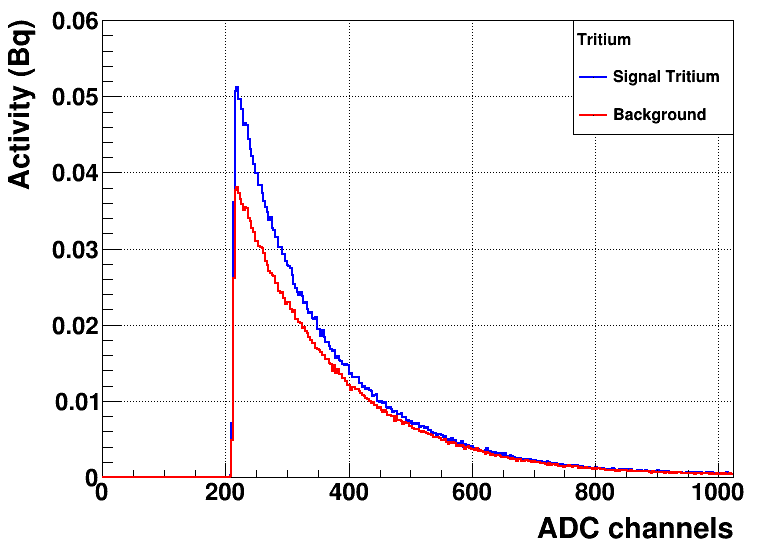
\includegraphics[scale=0.29]{tritio-fondo.png} 
}
{
%\subfloat[Espectro de emisión]
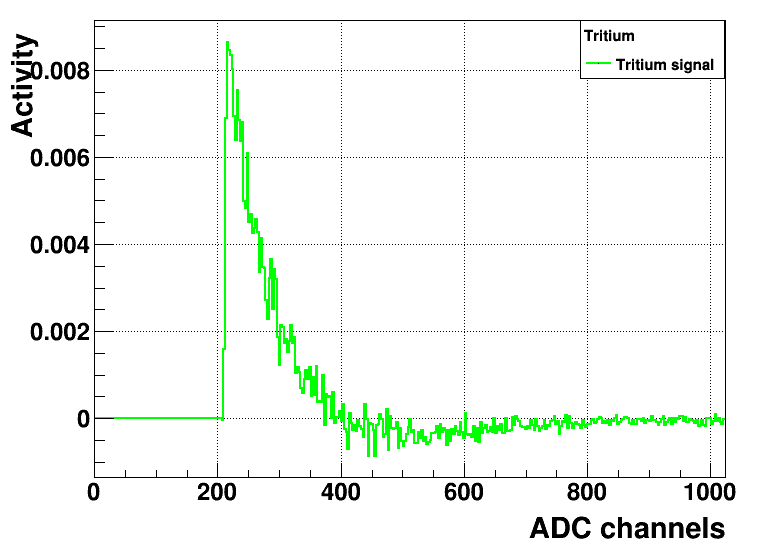
\includegraphics[scale=0.29]{tritiumsignal.png} 
}
\caption{Histograma energético de la señal del prototipo con tritio y del fondo superpuestos y señal únicamente debido al tritio.\label{senaltritio}}
\end{figure}


En esta figura podemos observar que estamos detectando un pico de señal de aproximadamente $0.0505 \pm 5.7 \cdot 10^{-4}~\becquerel$ y una señal debida únicamente a tritio de aproximadamente $0.0132 \pm 6.9 \cdot 10^{-4}~\becquerel$. 

Para ver hasta que punto nuestro sistema funciona de forma adecuada, podemos realizar un rápido cálculo para ver cual es la actividad que esperamos detectar con nuestro prototipo. Para ello, por un lado calculamos el volumen efectivo de la fuente (volumen de agua tritiada que  contribuye a la señal final) y, por otro lado, utilizamos este volumen para determinar cual es la actividad que deberíamos medir en nuestro experimento.

\begin{itemize}
 \item{} Para calcular el volumen efectivo de la fuente tenemos en cuenta que los electrones procedentes de la desintegración del tritio poseen un recorrido libre medio de $5~\micro\meter$. Por tanto, únicamente contribuirá de forma apreciable a la señal el agua tritiada que se encuentre en  un cilindro de grosor $5~\micro\meter$ alrededor de cada fibra. Pasamos a calcular este volumen. Para ello, calcularemos el volumen total y, a esta cantidad, le substraeremos el volumen ocupado por la fibra.

El volumen de la fibra es el volumen correspondiente a un cilindro de radio $0.5~\mm$ (radio de la fibra) y una longitud efectiva de $20~\cm$, donde se ha tenido en cuenta que, aunque la longitud real de la fibra son $25~\cm$, esta contiene en los extremos del haz unos aros metálicos y, además, parte de esta fibra sobresale del prototipo para acoplar a los PMTs. Por tanto, esta sección de la fibra, aproximadamente $2,5~\cm$ en cada extremo,  no contribuye a la señal del tritio. Con todo esto, el volumen ocupado por la fibra será $V_{fibra}=1.5708 \cdotp 10^{-4}$ litros.

Análogamente calculamos el volumen ocupado por la fuente más la fibra (volumen total), que corresponderá a un cilindro de radio $0.5~\mm+5\mu m$ (radio de la fibra + radio efectivo de la fuente) y la misma longitud que la fibra, es decir, $20~\cm$, ya que en estos extremos se encuentra el final del prototipo. Como resultado el volumen ocupado por la fibra y la parte de la fuente que contribuye a la señal de esta fibra es $V_{total}=1.6023 \cdotp 10^{-4}$ litros. 

Por tanto el volumen ocupado únicamente por el porcentaje de la fuente que esta interviniendo en la señal de esta fibra será la diferencia entre estos $V_{fuente}=3.1573 \cdotp 10^{-6}~\liter$.
 
Por tanto, teniendo en cuenta que el prototipo únicamente dispone de un haz formado por 35 fibras centelleadoras, el volumen efectivo final del agua tritiado que podemos detectar será el anterior multiplicado por 35, es decir, $1.1050 \cdotp 10^{-4}~\liter$. 

Hay que tener en cuenta que, en esta última multiplicación, se ha supuesto que el volumen de agua tritiada asociada a cada fibra forma un conjunto disjunto y sabemos que esto no es así ,ya que se producen solapamientos entre ellos. Debido a ello este cálculo será únicamente aproximado.

\item{} Ahora, procedemos a calcular la actividad del prototipo conociendo el volumen de agua tritiada que está aportando  la señal total. Para ello, tenemos en cuenta que la disolución contiene $2.0169 \pm 0.0017~\gram$ de tritio con una actividad específica de $26.8 \pm 0.6~\mega\becquerel/\gram$ disueltos en medio litro de agua hiperpura (Sec. $\ref{sec:Llenado}$). Con esto podemos calcularla actividad total de la disolución, que aproximadamente de $108.11~\mega\becquerel/\liter$. 

Por tanto, si en un litro hay aproximadamente $1.0811\cdotp 10^{8}$ desintegraciones por segundo, en el volumen calculado anteriormente habrá aproximadamente $1.1996\cdotp 10^{4}$ desintegraciones por segundo, es decir, $11.996~\kilo\becquerel$.

Finalmente, teniendo en cuenta que la eficiencia de la fibras y de los PMTs son, aproximadamente, 3\% y 30\% respectivamente y suponiendo que la cadena electrónica posee una eficiencia del $100\%$, llegamos a que la actividad que deberíamos detectar es, aproximadamente $107.96~\becquerel$.

\end{itemize}

Podemos ver que estamos detectando 4 ordenes de magnitud menos de lo que deberíamos. Esto es debido en parte a imperfecciones del sistema, pero la principal fuente de la pérdida de la señal es  el hecho de que las fibras empleadas en este prototipo no poseen clad. 

El clad hace que los fotones sean conducidos por el interior de las fibras a partir de reflexiones hasta el fotosensor, es decir, actúa como guía de luz. En nuestro caso, fibras sin clad, en cada reflexión se produce una pérdida del $94\%$ de la señal, por tanto, prácticamente la totalidad de los fotones de emisión de las fibras escaparán de estas, llegando al agua y produciendo de esta forma una pérdida de señal. 

Como resultado únicamente detectaremos el porcentaje asociado al ángulo sólido cubierto por las fibras centelleadoras respecto al total de electrones emitidos por el tritio, cuya emisión supondremos isótropa. Además, del total de fotones reemitidos por las fibras centelleadoras (de nuevo se supone emisión isótropa) ante la detección de este electrón, únicamente detectaremos el porcentaje asociado al ángulo sólido cubierto por la cara final de la fibra centelleadora. También hay que tener en cuenta que el porcentaje de fibra que se encuentra en la parte inferior de la U que constituye el prototipo apenas intervendrá en la señal, ya que vemos que prácticamente la totalidad de esta será perdida (su ángulo sólido es nulo). 

Podemos realizar una rápida estimación de la magnitud relativa de estos ángulos sólidos para ver su importancia en la pérdida de la señal. Integrando la expresión del ángulo sólido para una esfera, esta toma la siguiente forma: $\Omega=2\pi(1-\cos{\theta})$ donde $\theta$ es el ángulo que subtiende la superficie que queremos calcular~\cite{unizar}. Por tanto, dado que la superficie total de emisión será $4\pi$ ($\theta=180\degree$) el factor de reducción debido al ángulo sólido será:
\begin{equation}
\frac{\Omega}{4\pi}=\frac{1-\cos{\theta}}{2}
\label{factordebidoalangulosolido}
\end{equation}

Si  calculamos el ángulo y, por extensión, este factor para el caso del ángulo sólido subtendido por la fibra centelleadora, vemos que este ángulo siempre será aproximadamente $90\degree$ , debido al hecho que la fibra centelleadora es mucho mayor que su destancia al punto de la desintegración, $5\micro\meter$ como máximo. Por tanto, este factor será aproximadamente $0.5$ en todo momento, es decir, aproximadamente la mitad de los electrones que se producen en este punto del agua tritiada pasan por la fibra. Sin embargo, la transmisión de fotones por las fibras al detectar un electrón es un factor realmente pequeño. Por ejemplo, un punto situado a $2~\centi\meter$ de la cara final de la fibra, posee un factor de $3.12\cdotp 10^{-4}$, llegando a valer $0$ para los puntos correspondientes a la parte inferior del prototipo, como se ha mencionado anteriormente. Vemos por tanto, que si llega a ser un factor realmente relevante y que podría explicar la gran pérdida de señal observada. 

Por tanto, debido a la necesidad de recolectar el máximo de luz, un paso inmediato en el siguiente prototipo será incluir fibras con clad que nos permitan recolectar un mayor porcentaje de luz. El problema reside en que el grosor actual del single clad comercial de las fibras Saint-Gobain es de, aproximadamente, $4\%$ del diametro, es decir, $40~\mu m$. Prácticamente ningún electrón conseguirá pasar el clad y ser detectado en el núcleo de la fibra, por lo que habrá que considerar otros mecanismos de guía de ondas. Una posible solución a este problema es incluir nosotros el clad en las fibras a partir del proceso de deposición de aluminio por evaporación en vacío. Esto lo podemos realizar en el ICMOL, departamento vecino del IFIC, con el cual ya se han realizado trabajos similares anteriores~\cite{cladtesis,cladarticulo}. De esta forma, podríamos conseguir un clad con un espesor del orden de cientos de nanómetros, espesor suficientemente pequeño para que un porcentaje aceptable de electrones derivados de la desintegración del tritio puedan superarlo. 

En último lugar, para comprobar que nuestro argumento de la pérdida de la señal, situamos una fuente de actividad conocida, cuya emisión sea suficientemente energética, en el exterior del prototipo y procedemos a medir la señal. 

Si ahora también medimos una actividad con aproximadamente cuatro órdenes de magnitud inferior a la actividad teórica estipulada por la fuente, $3~\micro\curie \approx 1.11 \cdotp 10^{5}~\becquerel$, no habremos confirmado nuestro argumento, pero si le habremos dado mucho peso ya que, una vez los fotones emitidos por la fibra llegan al PMT ya es realmente complicado perder la señal. 

La fuente elegida es $\ce{^{137}Cs}$, el cual se desintegra $\beta^{-}$, según el siguiente esquema
\begin{equation}
\ce{^{137}Cs} \rightarrow \ce{^{137}Ba} + e^- + \overline{\nu}_e
\label{desintegracionbeta}
\end{equation}
cuyos electrones emitidos en esta desintegración poseen una energía promedio de $512~\kilo\eV$ ~\cite{Isotopos}. Estos electrones no llegaremos a verlos, pero tras esta desintegración el $\ce{^{137}Ba}$ se encuentra en un estado excitado y, por consiguiente, se desexcita en un tiempo de $153~\second$  a partir de una desintegración $\gamma$ cuyos fotones tienen una energía de $662~\kilo\eV$~cite{Isotopos}. Estos son los fotones que llegarán a la fibra centelleadoras y que pretendemos utilizar para obtener la eficiencia del sistema. Hay que tener en cuenta que, debido al pequeño tamaño de las fibras centelleadoras, únicamente aspiramos a detectar el valle Compton de esta desintegración, es decir, no conseguiremos observar el pico debido al efecto fotoeléctrico. Este valle Compton corresponde aproximadamente a un $10\%$ de las cuentas, es decir, únicamente aspiramos a detectar una actividad de $1.11 \cdotp 10^{4}~\becquerel$. Si además tenemos en cuenta la eficiencia de los PMTs y de las fibras centelleadoras, $30\%$ y $3\%$ respectivamente, únicamente aspiraremos a detectar una actividad de $99.9~\becquerel \approx 1 \cdotp 10^{2} \becquerel$

A continuación, de forma similar al caso del tritio, mostramos el espectro medido con el prototipo y la fuente de $\ce{^{137}Cs}$.

\begin{figure}[htb]
\centering
{
%\subfloat[Espectro de emisión]
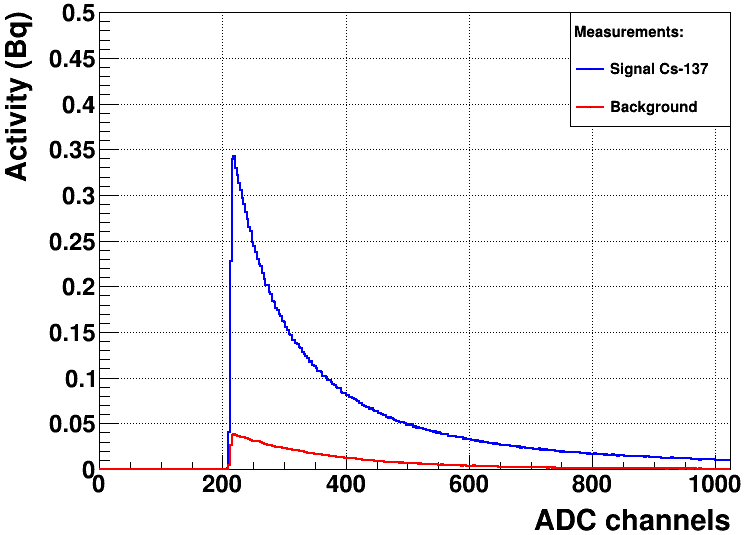
\includegraphics[scale=0.29]{Signal_Cs-137+background.png} 
}
{
%\subfloat[Espectro de emisión]
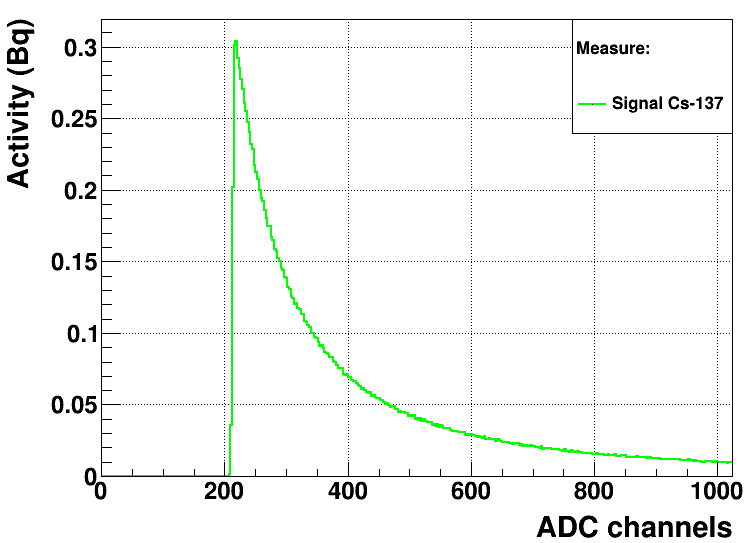
\includegraphics[scale=0.29]{Signal_Cs-137.png} 
}
\caption{Histograma energético de la señal del prototipo con fuente de $\ce{^{137}Cs}$ y del fondo superpuestos y señal únicamente debido al $\ce{^{137}Cs}$.\label{senalcesio}}
\end{figure}

En este espectro podemos ver que se ha medido una señal con una actividad aproximada de $0.305 \pm 1.6 \cdot 10^{-3}~\becquerel$. Vemos que se trata de aproximadamente 3 ordenes de magnitud por debajo de lo que esperaríamos detectar.

Por tanto, procedemos a calcular el ángulo sólido para verificar que su valor podría explicar esta diferencia. Para ello, por un lado suponemos que únicamente tienen aportación a la señal los fotones que llegan directamente de la fuente y justo en la cara final del haz son absorbidos por las fibras centelleadoras y convertidos en luzde centelleo,  ya que, por un lado, debido al espectro de la eficiencia de fotodetección de los PMTs, los fotones de $662~\kilo\eV$ que llegan al PMT no tendrán aportación significativa y, por otro lado, debido al ángulo sólido, los que se absorben a una distancia mínima de la cara final tampoco tendrán aportación. Además, tenemos en cuenta que la fuente se ha situado sobre la parte central de la U y debajo de la estructura de acero que sujeta el prototipo (fig. $\ref{prototipo}$).Con todo esto, el ángulo sólido calculado es aproximadamente $2.845 \cdotp 10^{-3}$. 

Vemos que este ángulo sólido justo nos aporta la diferencia de tres órdenes de magnitud que necesitamos. Tomando por válido nuestro argumento obtendríamos una señal máxima de $0.284~\becquerel$, la cual vemos que se acerca de forma aceptable al valor esperado.

Por tanto, aunque no hayamos comprobado que la pérdida de señal sea debida al ángulo sólido, vemos que es esta hipótesis se ajusta  a los resultados. Las mínimas desviaciones podrían ser debido a que se ha considerado que únicamente aportan a la señal los fotones detectados justo en la cara final. Esto ha sido una aproximación para realizar un rápido cálculo, pero realmente también tendrán aportación los fotones detectados a una distancia del orden del milímetro o inferior, lo cual se traduciría en un ligero aumento del ángulo sólido y por tanto, de la señal detectada. Este hecho podría explicar  el resultado obtenido en esta prueba de verificación. La prueba que nos confirmará en último lugar nuestra hipótesis será las simulaciones realizadas sobre el experimento.
